\documentclass[11pt,a4paper]{article}

\usepackage[utf8]{inputenc} 
\usepackage[T1]{fontenc} 
\usepackage{lmodern}
\usepackage[margin=2cm]{geometry}
\usepackage[german]{babel}
\usepackage{amsmath} 
\usepackage{graphicx} 
\usepackage{booktabs}
\usepackage{hyperref}
\hypersetup{
    colorlinks,
    citecolor=red,
    filecolor=black,
    linkcolor=black,
    urlcolor=black} 
\usepackage{nicefrac}
\usepackage[table]{xcolor}
\usepackage{tocloft}
\usepackage{wrapfig}
\usepackage[section]{placeins}

\setlength{\parindent}{0pt}
\setlength{\parskip}{1ex plus 0.5ex minus 0.5ex}

\definecolor{incolor}{rgb}{0.0, 0.0, 0.5}

\hbadness=99999

\newcommand{\refpy}[1]{Siehe Anhang: \textit{Rechnungen in Python} (\texttt{{\color{incolor}In [{\color{incolor}#1}]}})}
\newcommand\dif{\mathop{}\!\mathrm{d}}
\newcommand{\halftime}[4]{\begin{figure}[h]
\begin{minipage}{.#1\textwidth}#3\end{minipage}\begin{minipage}{.#2\textwidth}
\centering
#4\end{minipage}
\end{figure}}
\renewcommand{\vec}{\boldsymbol}
\newcommand{\biz}[2]{\bigg(\frac{#1}{#2}\bigg)}

\newcommand\mean{\begin{equation}
\frac{\sum_{i=1}^n x_i}{n}\label{mean}
\end{equation}}
\newcommand\meanstd{\begin{equation}
s_x=\sqrt{\frac{1}{n-1}\sum_{i=1}^n(x_i-\overline{x})^2}\label{meanstd}
\end{equation}}
\newcommand\prodquo{\begin{equation}\left\vert\frac{\Delta z}{z}\right\vert=\sqrt{\left(a\frac{\Delta x}{x}\right)^2+\left(b\frac{\Delta y}{y}\right)^2+\ldots}\textrm{ f\"ur }z=x^a\ y^b\ldots\end{equation}}
\newcommand\tfuncd{\begin{equation}
\frac{\vert x_n-y_n\vert}{\sqrt{x_s^2+y_s^2}}
\end{equation}}
\newcommand\tfunc{\begin{equation}
\frac{\vert x-y_0\vert}{u_x}
\end{equation}}

\begin{document}


{
\centering 
\large 
Physiklabor für Anf\"anger*innen \\
Ferienpraktikum im Sommersemester 2018 \\[4mm]
\textbf{\LARGE 
Versuch 23: Schallwellen
} \\[3mm]
(durchgef\"uhrt am 08.10.2018 bei Pascal Wunderlin) \\
Gruppe 14: Andréz Gockel\\ Gruppe: 13  Marouan Zouari\\
\today \\[10mm]
}

\vfill
\tableofcontents
\vfill
\pagebreak

\section{Ziel des Versuchs}
Dieser Versuch hat drei Teile die es ermöglichen die Schallgeschwindigkeit durch drei verschiedene Verfahren zu bestimmen. In dem ersten Teil wird mit einem Quinckeschen Rohr die abstände der Minima und Maxima der Schallwelle bestimmt. In dem zweiten teil wird mit einem Sender und entgegengesetztem Empfänger mittels Oszilloskop die Wellenlänge gemessen. In dem dritten Teil wird Sender und Empfänger nebeneinander gesetzt und gegen eine Fläche gerichtet, dann wird mit dem Oszilloskop die Zeit gemessen die die Welle braucht um reflektiert zu werden und wieder zum Empfänger zu gelangen.

\section{Teil 1}

\subsection{Aufbau}

\begin{wrapfigure}{h}{.18\textwidth}
	\centering \vspace{-20pt}
	\fbox{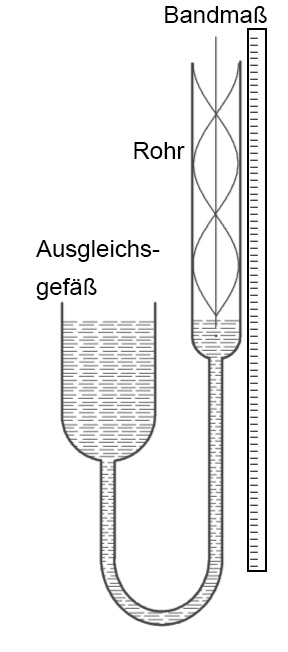
\includegraphics[scale=0.5]{Abb1}}
	\vspace{-5pt}
	\caption{Quinckesche Rohr \cite{Anleitung}}
	\label{abb1}
\end{wrapfigure}

In diesem Teil wird ein Quinckesches Rohr verwendet: dies besteht aus einem Lautsprecher und Mikrofon die über dem Rohr und auf das Wasser gerichtet. Die Wasserhöhe kann mit einer Centimeterskala die an dem Rohr befestigt ist abgelesen werden, die Wasserhöhe wird mit einem Ausgleichsgefäß bestimmt (siehe Abbildung \ref{abb1}) dessen höhe mit einer Kurbel verstellt wird.

 Hier ist zu beachten, dass das einstellen der Höhe eine Verzögerung hat. Der Lautsprecher ist an einem Frequenzgenerator verbunden, hiermit kann die Tonfrequenz eingestellt werden. Lautsprecher und Mikrofon sind mit einem Oszilloskop verbunden der es ermöglicht die Minima und Maxima auch visuell zu bestimmen. 


\subsection{Durchführung}

Als erstes wird eine beliebige Frequenz zwischen 2\,kHz und 7\,kHz eingestellt und Wasserhöhe zum Nullpunkt gebracht. Dann wird der Wasserspiegel gesunken bis sich ein Maxima bemerkbar macht und die entsprechende Höhe wird notiert. Es ist zu beachten, dass das Oszilloskop richtig eingestellt ist um die Maxima zu erkennen. Dies wird für mehrere Maxima wiederholt, dann wird die Frequenz geändert um eine weitere Reihe von Maxima zu messen. Dies wurde für drei Messreihen durchgeführt. 

\subsection{Auswertung}

Aus den Messwerten in Tabelle \ref{Tab:1} wird eine lineare Regression durchgeführt mit den Lagen $l_k$ über den Maxima $k$. Die Fitfunktionen sind 
\begin{align*}
	a_1 + b_1 x &= 3.3(9) + 7.6(3)x\\
	a_2 + b_2 x &= 3.1(9) + 4.1(4)x\\
	a_3 + b_3 x &= 5.29(7) + 2.57(1)x\\
\end{align*}

Welche mit

$$a=\frac{\sum x_i^2\sum y_i-\sum x_i\sum x_iy_i}{n\sum x_i^2-(\sum x_i)^2}$$
$$b=\frac{n\sum x_iy_i-\sum x_i\sum y_i}{n\sum x_i^2-(\sum x_i)^2}.$$
berechnet wurden und deren Unsicherheiten wurde mit der Streuung $s$ berechnet:

$$s =\sqrt{\frac{1}{n-2}\sum^n_{i=1}[y_i-(a+bx_i)]^2}$$

$$\Delta a=s\sqrt{\frac{\sum x_i^2}{n\sum x_i^2-(\sum x_i)^2}}$$

$$\Delta b=s\sqrt{\frac{n}{n\sum x_i^2-(\sum x_i)^2}}$$

Mit der Frequenz $\nu$ und der Steigung die eine halbe Wellenlänge $\lambda$ entspricht kann man nun die Gleichung für die Schallgeschwindigkeit in Luft $c_L$ lösen. $c_L = \nu \lambda$ 

\begin{align*}
	c_{L_1} &= 330(13)\, \nicefrac{\textrm{m}}{\textrm{s}}\\
	c_{L_2} &= 343(33)\, \nicefrac{\textrm{m}}{\textrm{s}}\\
	c_{L_3} &= 339.8(13)\, \nicefrac{\textrm{m}}{\textrm{s}}\\
	\overline{c_L} &= 338(12)\, \nicefrac{\textrm{m}}{\textrm{s}}
\end{align*}

Wobei die Unsicherheit hier die Standardabweichung des Mittelwerts ist:

$$s_{\overline{c_L}} = \frac{1}{\sqrt{n}} \sqrt{\frac{\sum_{i=1}^{n}(c_{L_i}-\overline{c_L})^2}{n-1}}$$

\subsection{Diskussion}

\pagebreak
\section{Teil 2}

\subsection{Aufbau}

\begin{wrapfigure}{h}{.4\textwidth}
	\centering \vspace{-20pt}
	\fbox{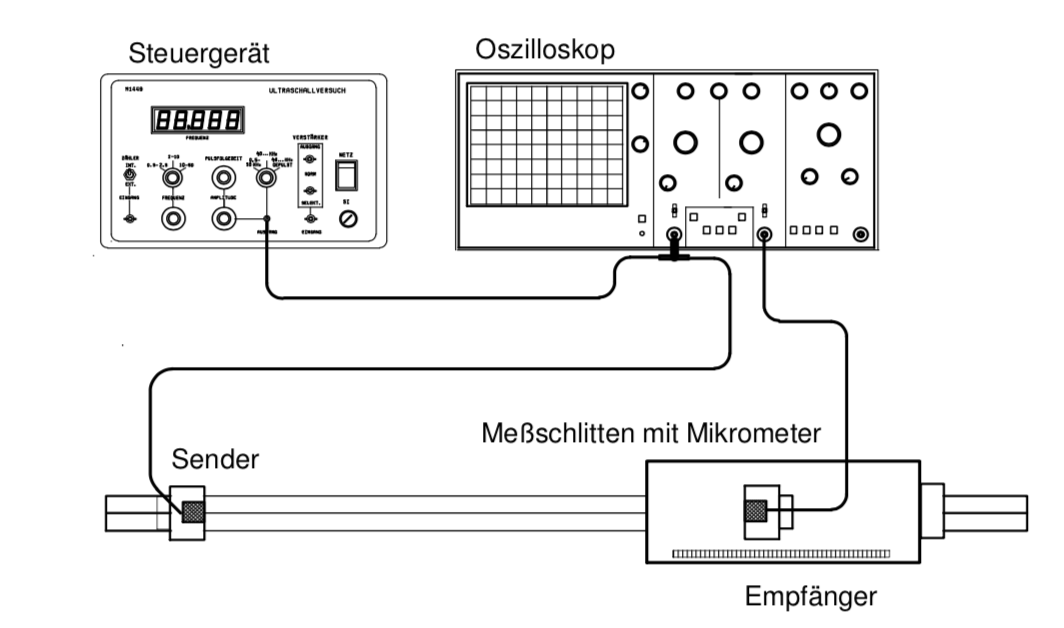
\includegraphics[scale=0.35]{Abb2}}
	\vspace{-5pt}
	\caption{Aufbau für Teil 2 \cite{Anleitung}}
	\label{abb2}
\end{wrapfigure}

Der Aufbau vom zweiten Teil besteht aus den folgenden Komponenten:
ein Ultraschallsender und -Empfänger, ein Oszilloskop, ein Signalgenerator und eine Bank mit Zentimeterskala worauf eine Halterung für den Sender und eine durch Mikrometerschraube verstellbare Halterung für den Empfänger platziert werden können. 

Der Sender und Empfänger werden so platziert, dass sie auf einander Zeigen. Hier ist zu Beachten, dass der Sender weg von der Wand zeigt um Störung durch Reflektionen zu vermeiden. Mittels der  Mikrometerschraube kann der Abstand zwischen Sender und Empf"anger variiert und die genaue Position notiert werden. Das Oszilloskop, woran beide Sender und Empf"anger angeschlossen sind, ermöglicht die Beobachtung der Ultraschallwellen.

\subsection{Durchführung}

Der Signalgenerator wurde Eingeschaltet und auf ein durchgehendes in dem 40\,kHz Frequenzbereich Ton geschalltet. Anschliessend wurde der Oszilloskop angeschaltet und justiert, sodass beide Signale im Bildschirm zu sehen waren. 

Mittels der Mikrometerschraube wird der Empfänger verschoben, bis die zwei angezeigten Signale in dem Oszilloskop überlagert waren. Dann wurde Seine Position notiert. Bei einer fixierten Startposition von der Empfängerhalterung wurden neun weitere Überlagerungen notiert. Dies wurde für vier verschiedene Startpositionen wiederholt. 

\subsection{Auswertung}

Die vier Messreihen wurden in einem in einer Graphik eingetragen: Abbildung \ref{uppy}. Dann wurden Ausgleichsgeraden eingesetzt dessen Steigung die Wellenlänge entspricht. Die Werte in der dritten Messreihe sind offensichtlich fehlerhaft und wir vermuten, dass Empfänger und Sender zu nah zu einander waren und das Oszilloskop welches eine gemittelte Kurve anzeigte durch reflektionen verwirrt wurde. Aus diesem Grund wird diese Messreihe aus der Mittelwertsrechnung gelassen. Wie in Teil 1 wird die Gleichung $c_L = \nu \lambda$ benutzt. Die Frequenz ist in dem Bereich von $\pm10\,$Hz geschwankt. 

$$\overline{c_L} = 345.5(3)\,\nicefrac{\textrm{m}}{\textrm{s}}$$

Für die Unsicherheiten der Schallgeschwindigkeiten wurde die vereinfachte Gaußsche Fehlerfortpflanzung für Produkte benutzt, aber da die Beträge von $\frac{u_\lambda}{\lambda}$ wesentlich größer als die $\frac{u_\nu}{\nu}$ Terme waren, wurden diese vernachlässigt:
$$ u_c = \left| \frac{u_\lambda}{\lambda}\right|$$
Die Unsicherheit des Mittelwerts wurde wie in Teil 1 berechnet:
$$s_{\overline{c_L}} = \frac{1}{\sqrt{n}} \sqrt{\frac{\sum_{i=1}^{n}(c_{L_i}-\overline{c_L})^2}{n-1}}$$

\subsection{Diskussion}

\pagebreak
\section{Teil 3}

\subsection{Aufbau}

\begin{wrapfigure}{h}{.5\textwidth}
	\centering \vspace{-20pt}
	\fbox{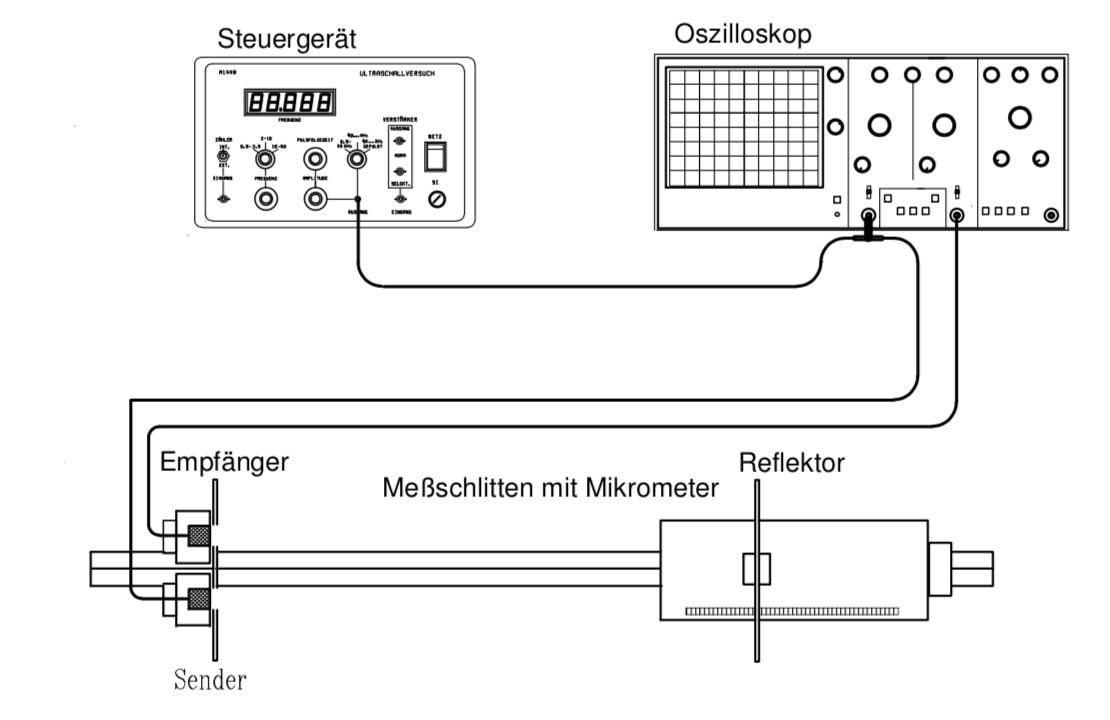
\includegraphics[scale=0.35]{Abb3}}
	\vspace{-5pt}
	\caption{Aufbau für Teil 3 \cite{Anleitung}}
	\label{abb3}
\end{wrapfigure}

In diesem Versuchsteil wird ein ähnlicher Aufbau wie in Teil 2 Verwendet, aber Sender und Empfänger werden in einer Platte parallel montiert, und sie zeigen auf eine geschlossene Platte die als Reflektor dient. Für die Messungen ist zusätzlich ein Massband benötigt. 

\subsection{Durchführung}

Der Signalgenerator wurde jetzt auf ein gepulsten 40\,kHz Ton gestellt, dieser wird nach 25 Schwingungen für 50\,ms blockiert. und auf ein durchgehendes in dem Das Oszilloskop wurde dann anders eingestellt, sodass der Anfang von einem puls, und der Anfang von der empfangenen Reflexion gut zu erkennen waren. Mit dem Massband wurden die Abstände zwischen der Platte mit dem Empfänger und Sender und der Reflektor Platte gemessen. Die Zeitdauer zwischen der ausgesandten Schallwelle und reflektierter Schallwelle wurde dann mit dem Oszilloskop für 10 verschiedene Abstände gemessen.

\subsection{Auswertung}

Die Schallgeschwindigkeit wird in diesem Teil bestimmt in dem die Abstände (wobei die gemessenen Abstände erst verdoppelt werden müssen) gegen die Zeit in einem Diagramm eingetragen werden, und mittels lineare Regression die Steigung bestimmt. (Abbildung \ref{durp}) 

Steigung aus der linearen Regression ist: $347$
Hierraus ergibt sich die Schallgeschwindigkeit:
$$c_L = 347(4)\,\nicefrac{\textrm{m}}{\textrm{s}}$$

Wobei die Streuung der Messwerte mit
$$s =\sqrt{\frac{1}{n-2}\sum^n_{i=1}[y_i-(a+bx_i)]^2} = 0.017$$
berechnet wurde und hiermit die Unsicherheit der Steigung bestimmt wurde:
$$\Delta b=s\sqrt{\frac{n}{n\sum x_i^2-(\sum x_i)^2}} = 3.7$$

\subsection{Diskussion}


\vfill

\begin{thebibliography}{9}
	\bibitem{Anleitung} Physikalisches Institut der Albert-Ludwigs-Universität Freiburg (Hrsg.) (08/2018): Versuchsanleitungen zum Physiklabor für Anfänger*innen, Teil 1, Ferienpraktikum im Sommersemester 2018.
\end{thebibliography}

\pagebreak

\section{Anhang}

\begin{table}[h]
	\centering
	\caption{Messwerte aus Teil 1} \vspace{11pt}
	$\begin{array}{l}
		\textrm{Unsicherheiten:}\\
		\textrm{Wasserhöhe: } \pm 0.5\, \textrm{cm}\\
		\textrm{Frequenz 1: } \pm 1\, \textrm{Hz}\\
		\textrm{Frequenz 2: } \pm 0.5\, \textrm{Hz}\\
		\textrm{Frequenz 3: } \pm 0.5\, \textrm{Hz}\\
	\end{array}$
	\begin{tabular}{cccc}
		\toprule
		\textrm{Start Frequenz} & 2176\,\textrm{Hz} & 4186\,\textrm{Hz} & 6610\,\textrm{Hz} \\
		\textrm{Stopp Frequenz} & 2173\,\textrm{Hz} & 4186\,\textrm{Hz} & 6610\,\textrm{Hz} \\
		\midrule 
		\textrm{Maxima $k$} & \multicolumn{3}{c}{\textrm{Lage $l_k$ in cm}} \\ 
		\midrule 
		1 & 11.1 &\ 7.0 &\ 8.0 \\
		2 & 18.5 & 11.5 & 10.5 \\
		3 & 25.5 & 15.5 & 13.0 \\
		4 & 35.0 & 19.5 & 15.5 \\
		5 & 41.0 & 23.5 & 18.0 \\ 
		6 & 	 & 27.5 & 20.6 \\ 
		7 & 	 & 31.5 & 23.5 \\
		8 &		 & 35.5 & 25.8 \\
		9 & 	 & 40.0 & 28.5 \\
		10&		 & 44.0 & 31.0 \\
		11& 	 &		& 33.7 \\
		12& 	 &		& 36.2 \\
		\bottomrule
	\end{tabular}
	\phantom{$\begin{array}{l}
		\textrm{Unsicherheiten:}\\
		\textrm{Wasserhöhe: } \pm 0.5\, \textrm{cm}\\
		\textrm{Frequenz 1: } \pm 1\, \textrm{Hz}\\
		\textrm{Frequenz 2: } \pm 0.5\, \textrm{Hz}\\
		\textrm{Frequenz 3: } \pm 0.5\, \textrm{Hz}\\
	\end{array}$}
	\label{Tab:1}
\end{table}

\pagebreak

\begin{figure}
\centering
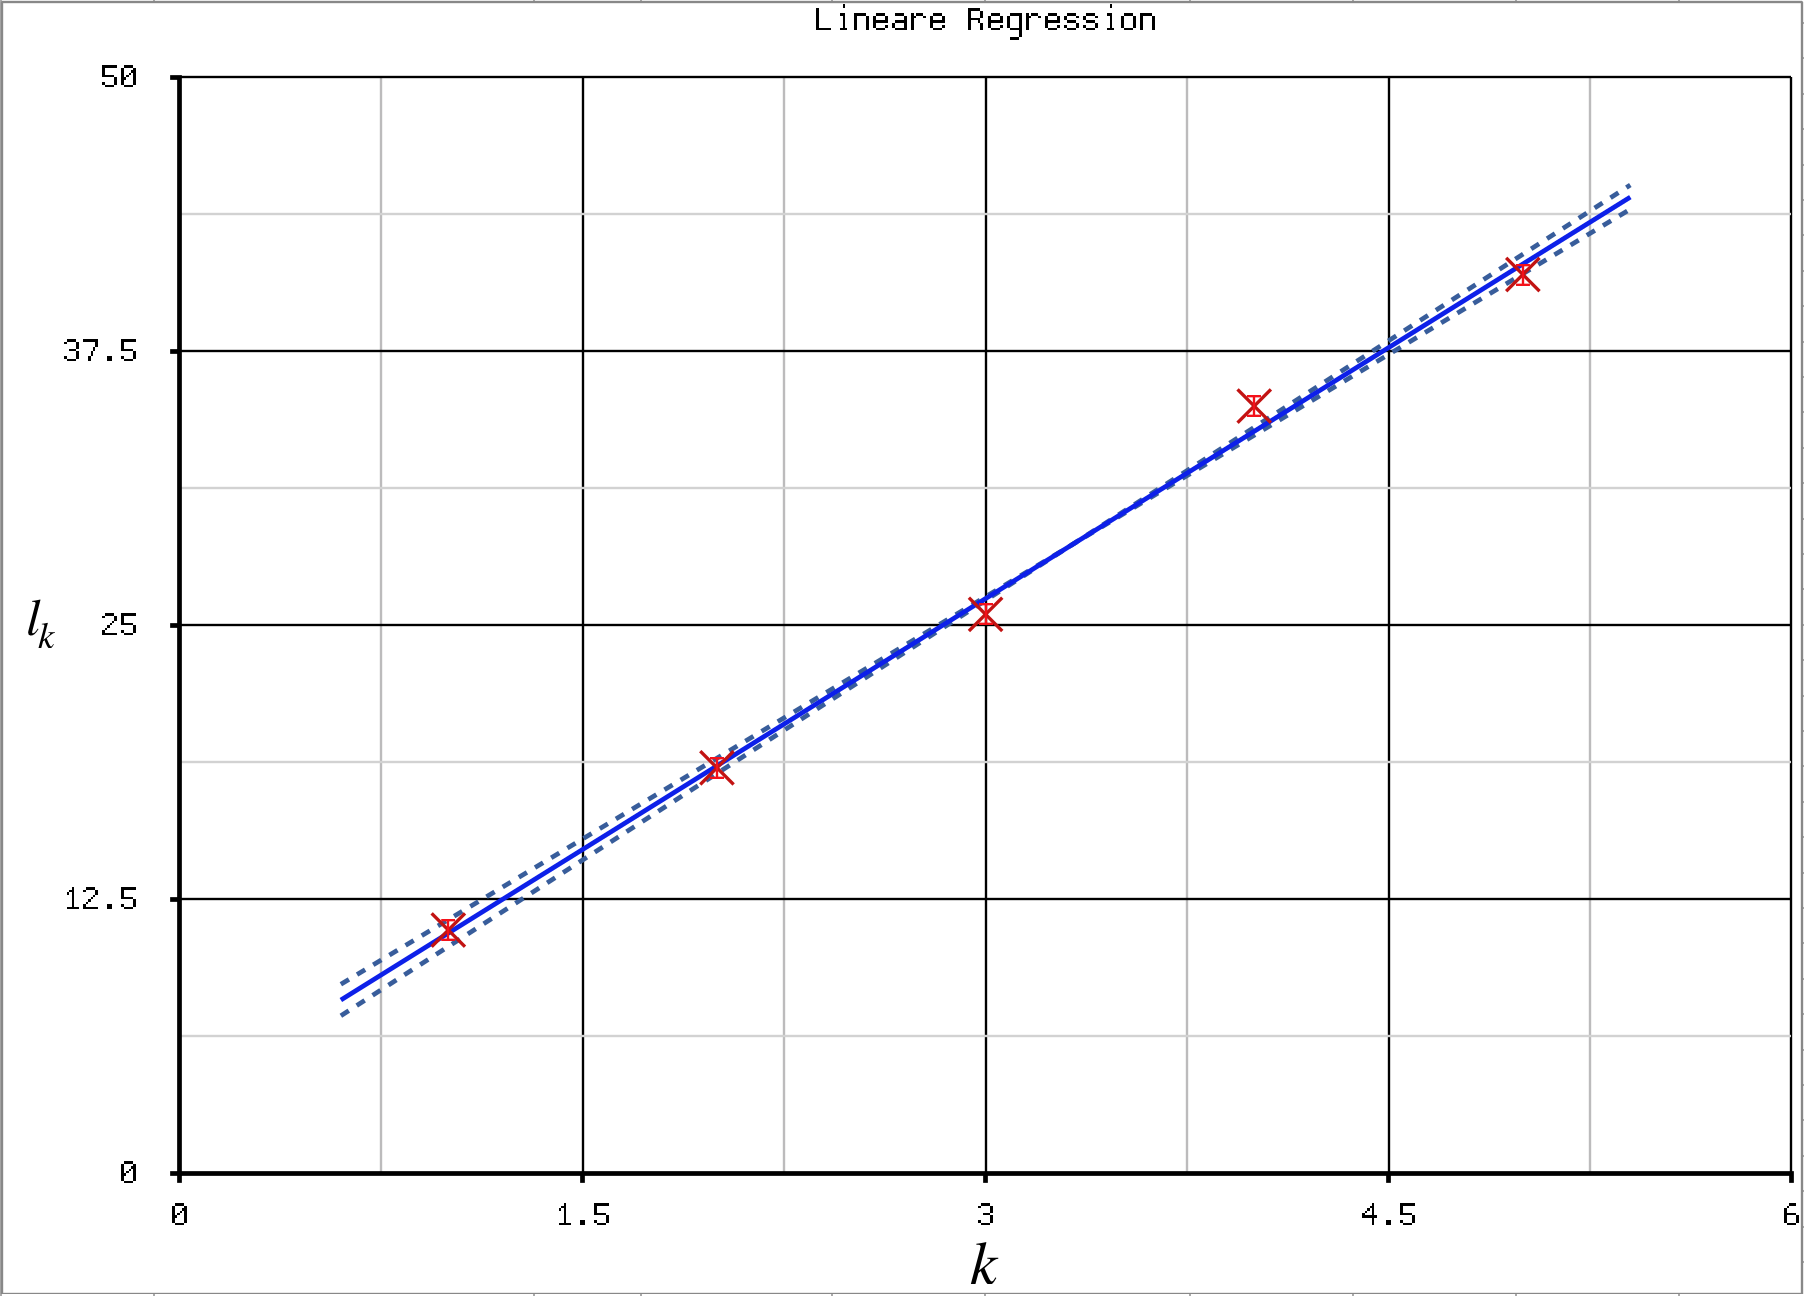
\includegraphics[width=.8\textwidth]{reg1}
\caption{2176\,Hz - 2173\,Hz}
\end{figure}

\begin{figure}
\centering
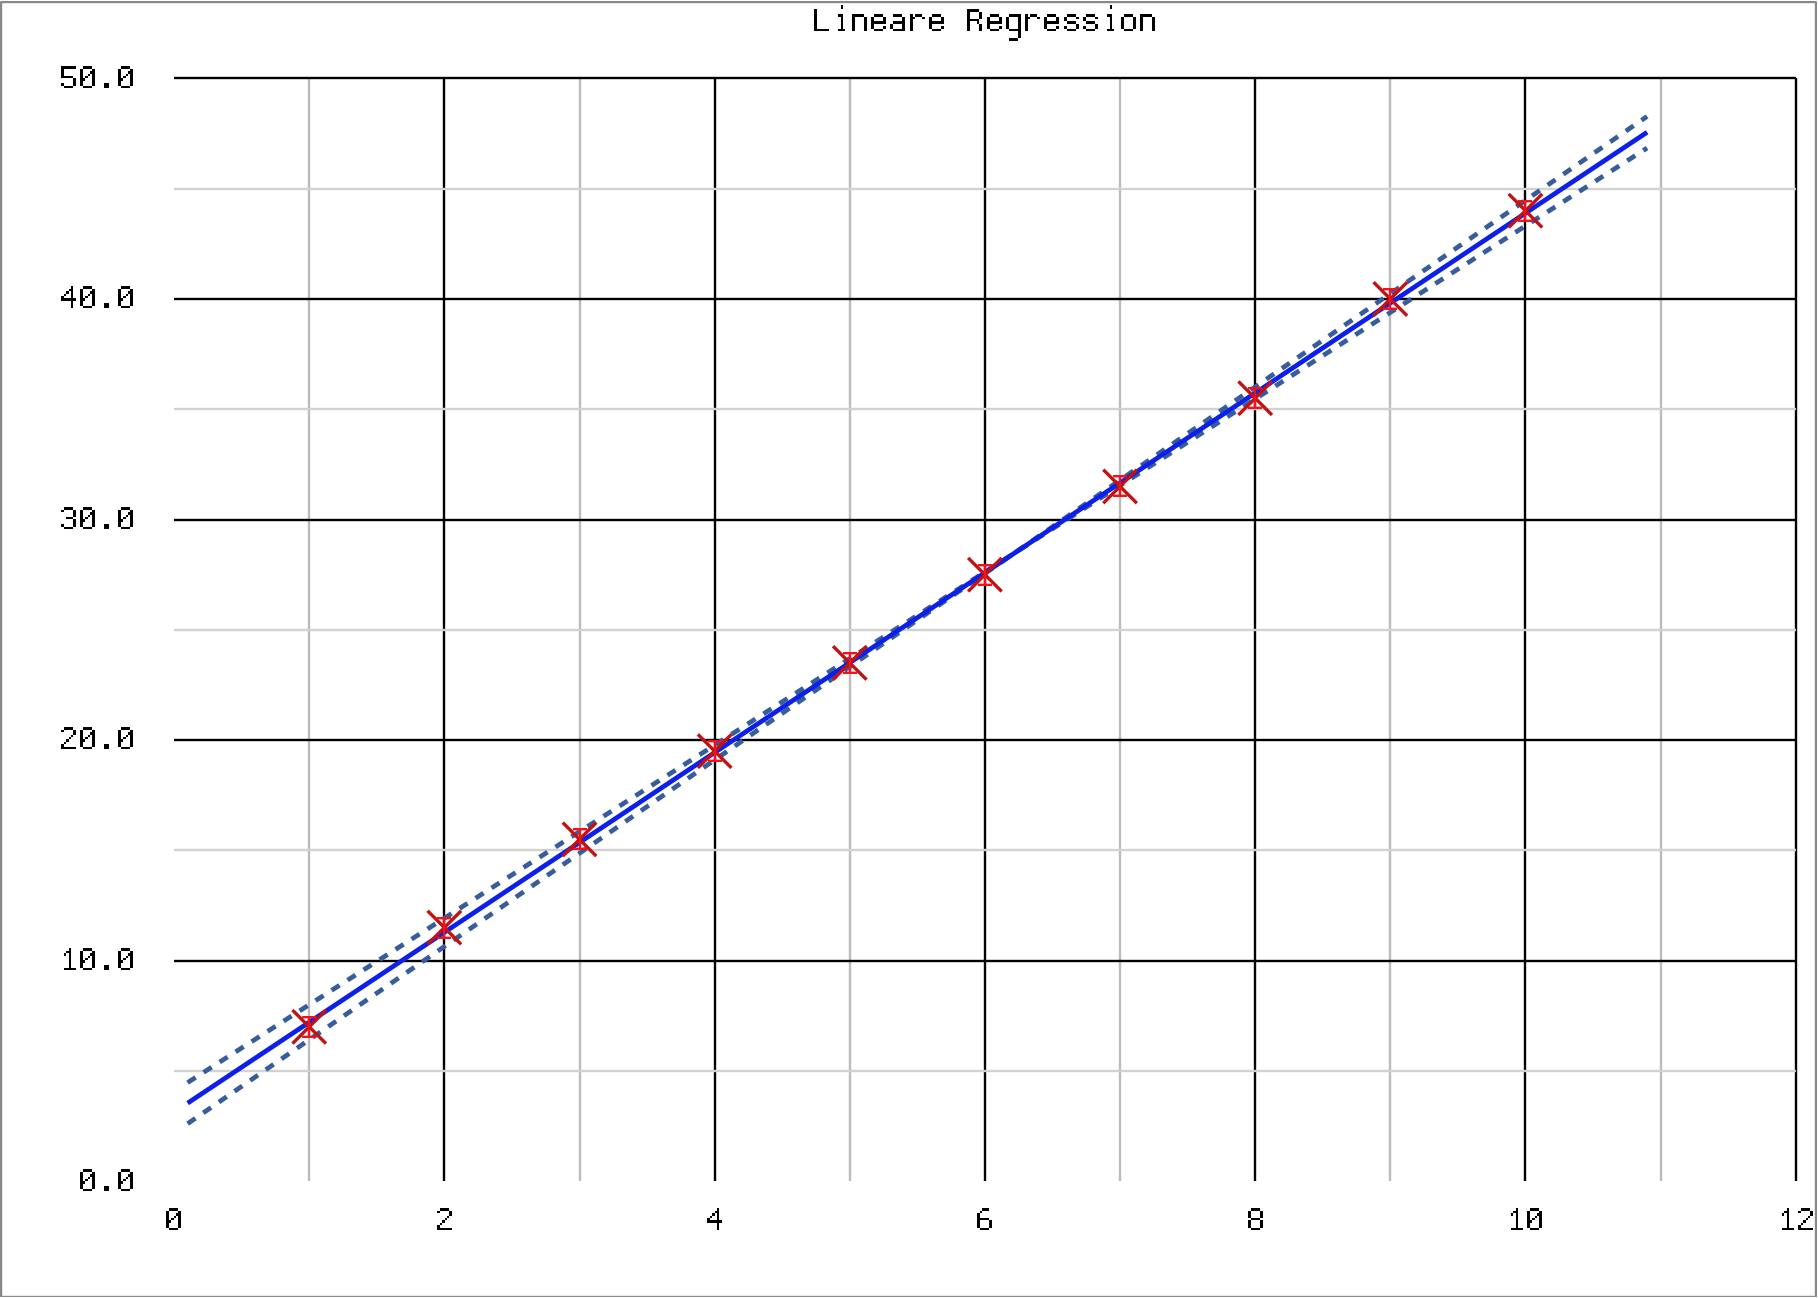
\includegraphics[width=.8\textwidth]{reg2}
\caption{4186\,Hz}
\end{figure}

\begin{figure}
\centering
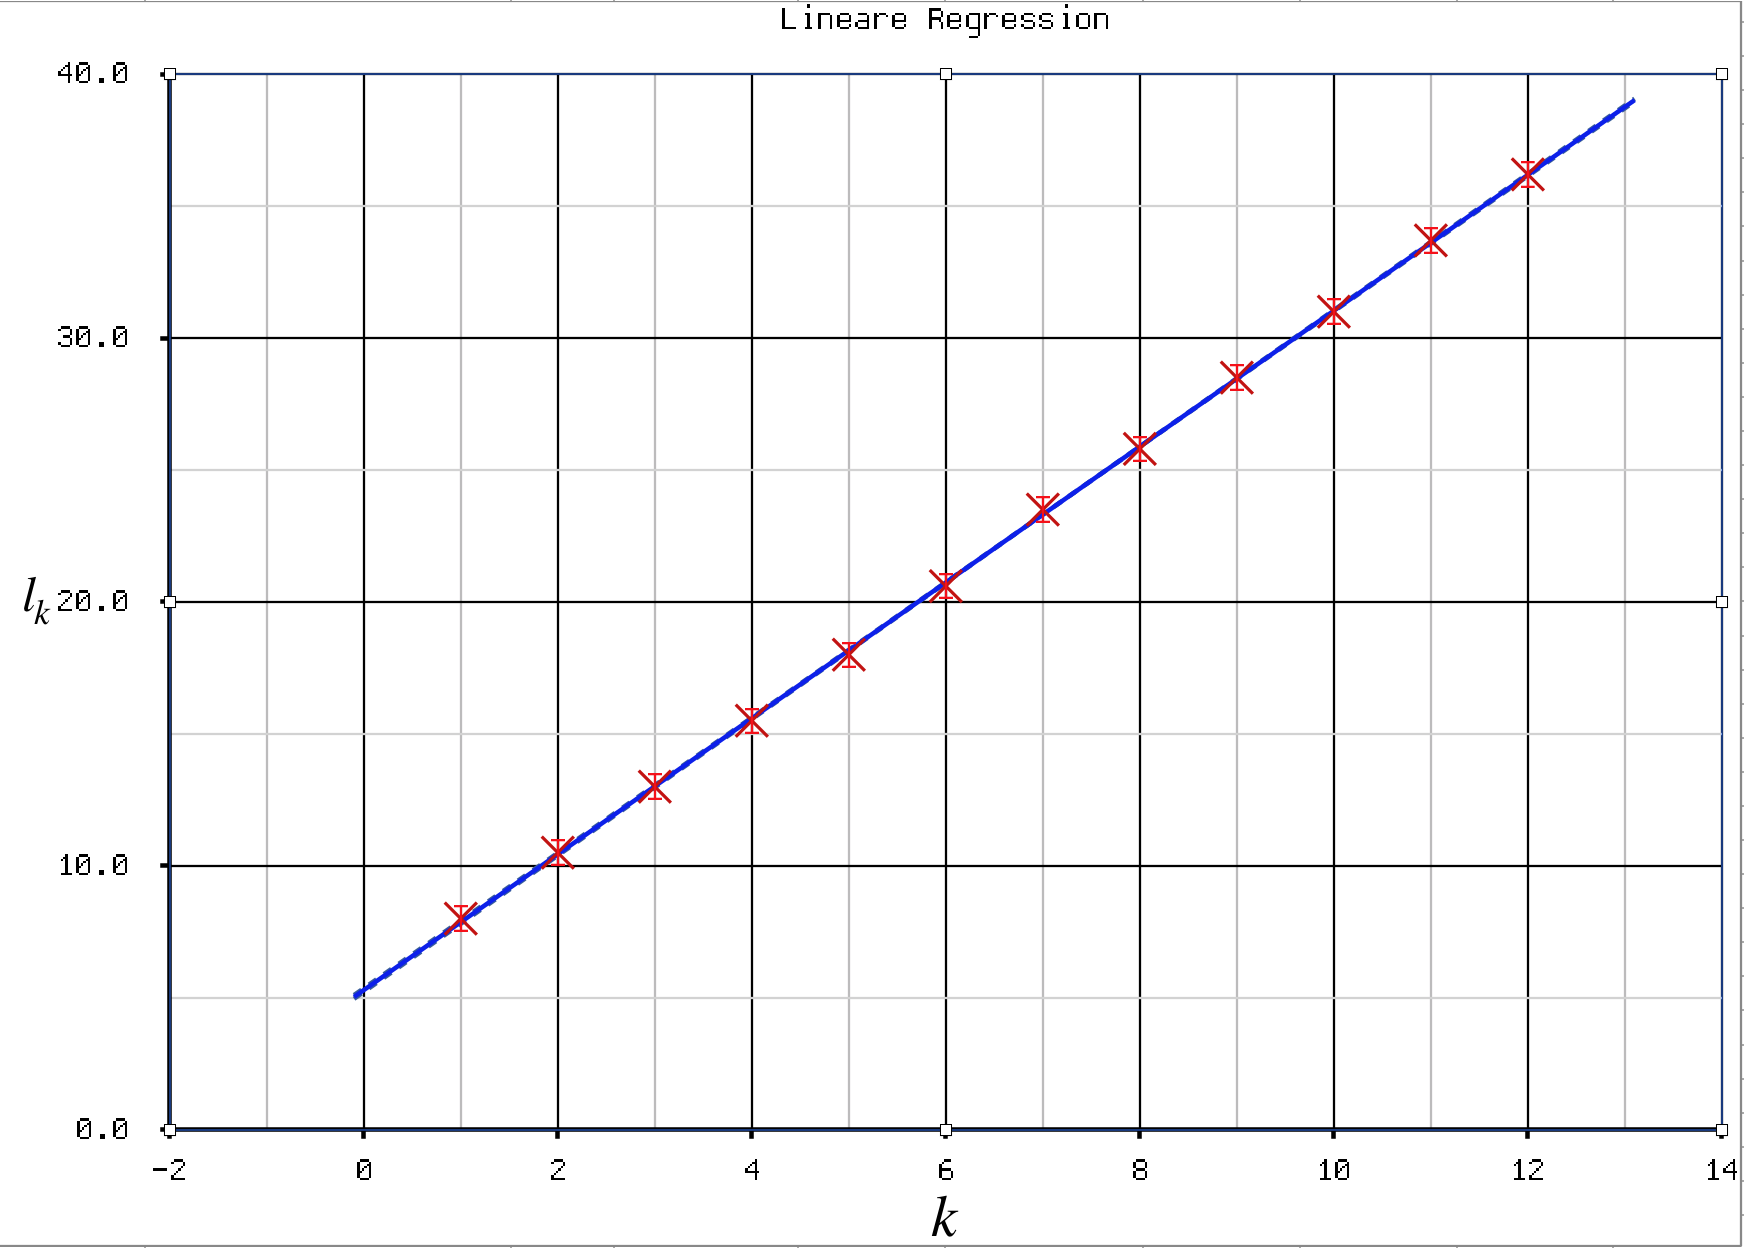
\includegraphics[width=\textwidth]{reg3}
\caption{6610\,Hz}
\end{figure}

\begin{figure}
\centering
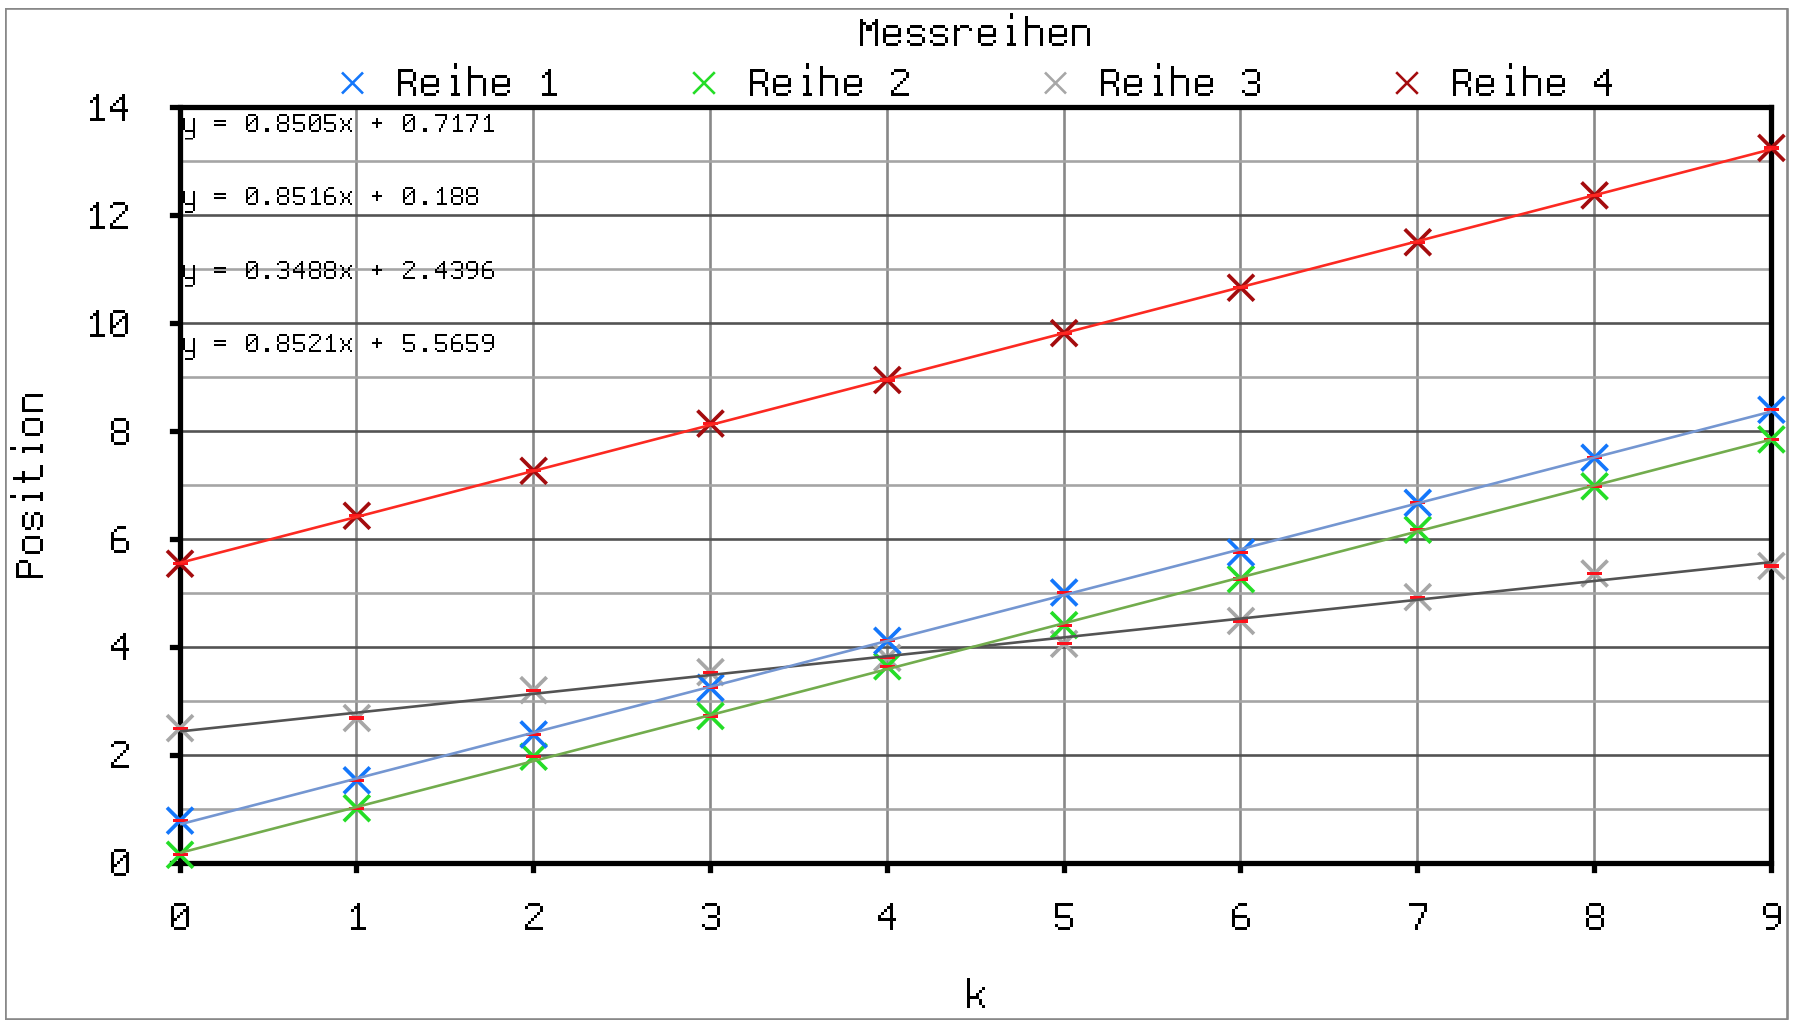
\includegraphics[width=\textwidth]{rect}
\caption{Ausgleichslinien Teil 2}
\label{uppy}
\end{figure}

\begin{figure}
\centering
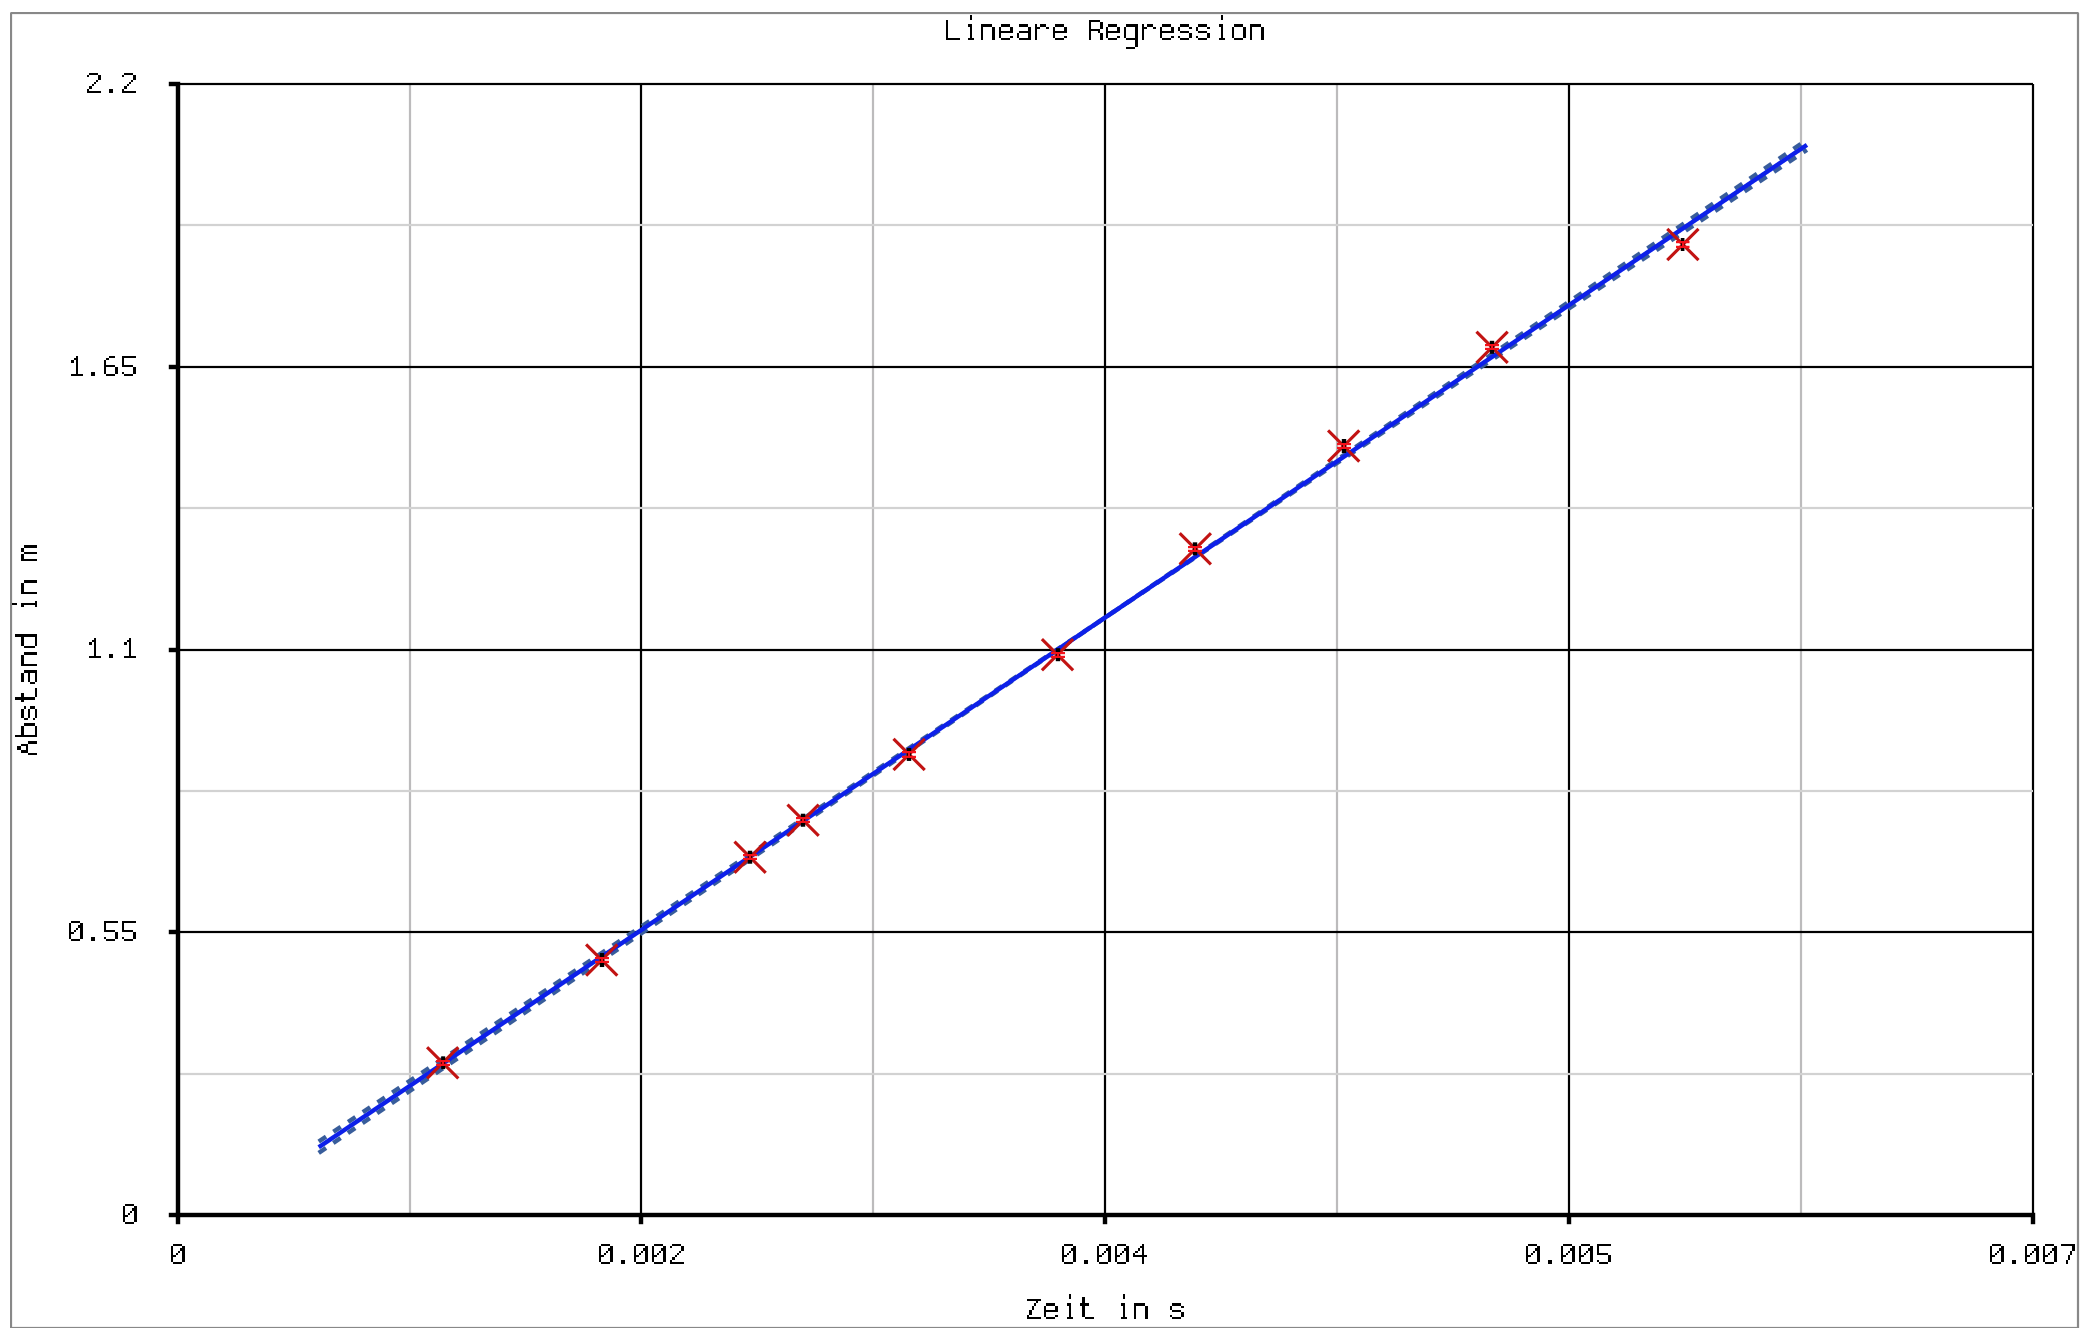
\includegraphics[width=\textwidth]{recd}
\caption{Lineare Regression Teil 3 (Fehlerbalken sind sehr klein und deswegen schwer zu sehen)}
\label{durp}
\end{figure}

\end{document}